\documentclass[12pt,a4paper]{article}

% Packages
\usepackage{graphicx}
\usepackage{amsmath}
\usepackage{listings}
\usepackage{textcomp}
\usepackage{caption}
\usepackage[top=1in,bottom=1in,left=1in,right=1in]{geometry}
\usepackage{fancyhdr}
\usepackage{float}
\usepackage{url}
\pagestyle{fancy}
\fancyhf{}
\rhead{Cadence Virtuoso Simulations}
\lhead{I-V Characterization}
\rfoot{Page \thepage}

% Listings configuration
\lstset{
  basicstyle=\ttfamily\small,
  columns=fullflexible,
  keepspaces=true,
  breaklines=true,
  captionpos=b
}

% Title
\title{LabReport 1}
\author{Arnav Yadnopavit\\EE24BTECH11007}
\date{August 2025}

\begin{document}
\maketitle

\section*{Aim}
To characterize the electrical behavior of a Diode, BJT, and MOSFET by plotting their I-V characteristics using Cadence Virtuoso simulations and standard SPICE models.

\section*{Apparatus}
\begin{itemize}
    \item Cadence Virtuoso Suite with Spectre Simulator
    \item Commercially available SPICE models:
    \begin{itemize}
        \item 1N4148 Diode
        \item 2N3904 NPN BJT
        \item 2N3906 PNP BJT
        \item 2N7000 N-channel MOSFET
    \end{itemize}
\end{itemize}

\section*{Theory}
\subsection*{1. Diode}
A diode allows current to flow in one direction and blocks it in the reverse. The I-V characteristic shows exponential rise in forward bias and negligible reverse current until breakdown.

\subsection*{2. BJT (Bipolar Junction Transistor)}
A BJT has three terminals: emitter, base, and collector. Its operation depends on base-emitter voltage and collector-emitter voltage. The output characteristic \( I_C \) vs \( V_{CE} \) is plotted at constant \( I_B \).

\subsection*{3. MOSFET (Metal-Oxide Semiconductor FET)}
MOSFETs operate in cutoff, linear, and saturation regions. The drain current \( I_D \) vs drain-source voltage \( V_{DS} \) is plotted for various gate-source voltages \( V_{GS} \).

\section*{Circuit Diagrams}
\subsection*{1. Diode I-V Characterization}
Forward bias circuit with DC voltage sweep.
\begin{figure}[H]
    \centering
    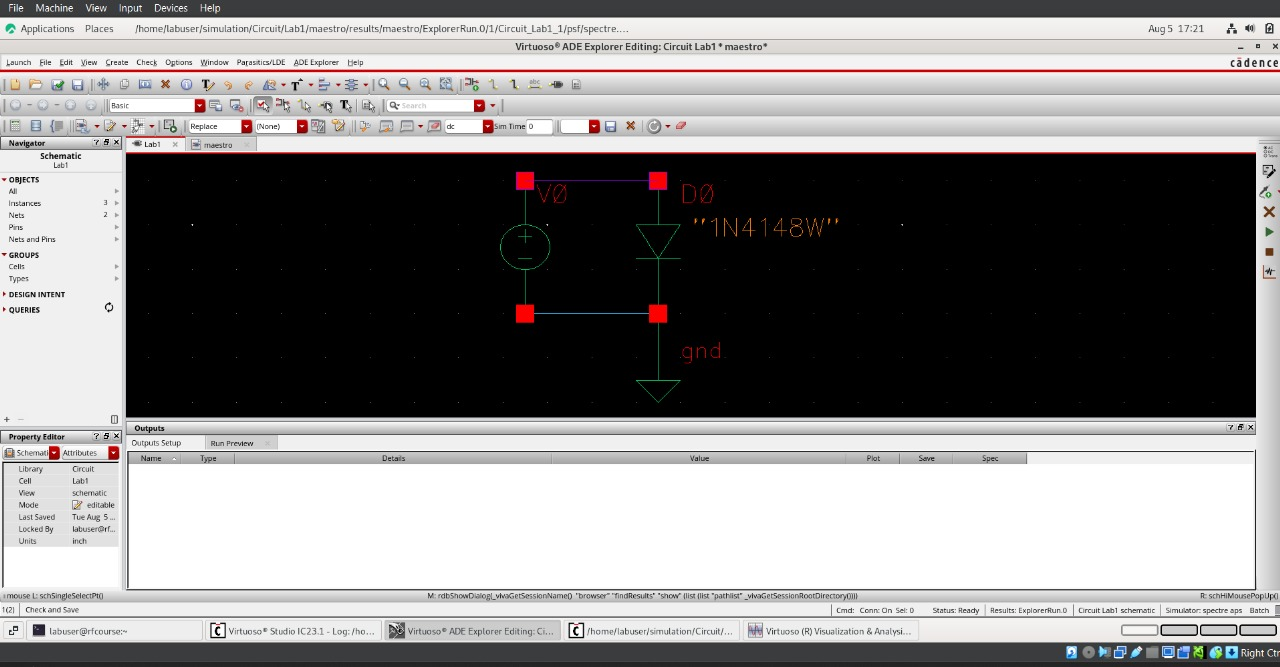
\includegraphics[width=\textwidth]{figs/Diode/Circuit.jpg} % Add your image file
    \caption{Circuit for Diode I-V Characterization}
\end{figure}

\subsection*{2. BJT I-V Characterization}
DC sweep of \( V_{CE} \) for multiple \( I_B \) values.
\begin{figure}[H]
    \centering
    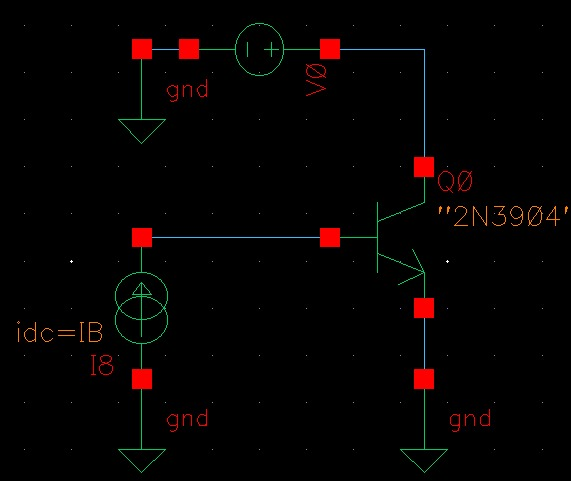
\includegraphics[width=0.7\textwidth]{figs/BJT/NPN/Circuit.jpg} % Add your image file
    \caption{Circuit for NPN BJT I-V Characterization}
\end{figure}
\begin{figure}[H]
    \centering
    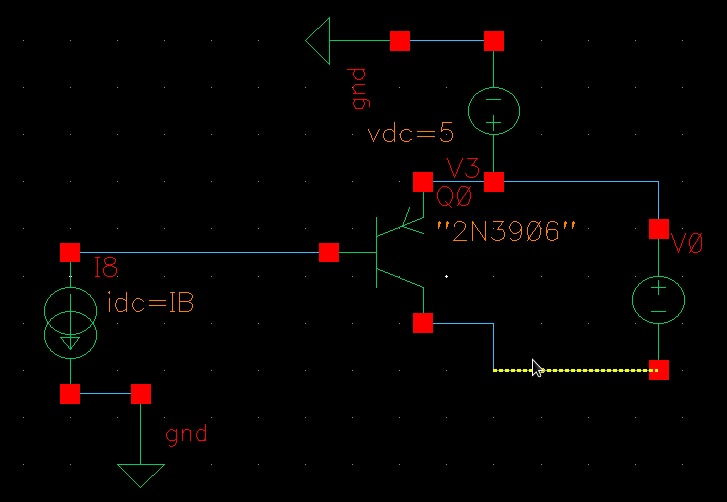
\includegraphics[width=0.7\textwidth]{figs/BJT/PNP/Circuit.jpg} % Add your image file
    \caption{Circuit for PNP BJT I-V Characterization}
\end{figure}
\subsection*{3. MOSFET I-V Characterization}
DC sweep of \( V_{DS} \)($V_0$) for multiple \( V_{GS} \) ($V_1$) values.
\begin{figure}[H]
    \centering
    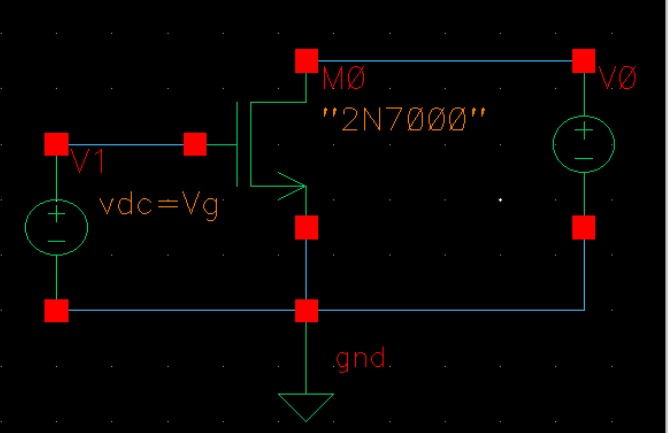
\includegraphics[width=0.7\textwidth]{figs/Mosfet/Circuit.jpg} % Add your image file
    \caption{Circuit for Mosfet I-V Characterization}
\end{figure}


\section*{SPICE Models}
For Spice Models refer to\\
\url{}

\section*{Observations}
\subsection*{1. Diode I-V Plot}
\begin{figure}[H]
    \centering
    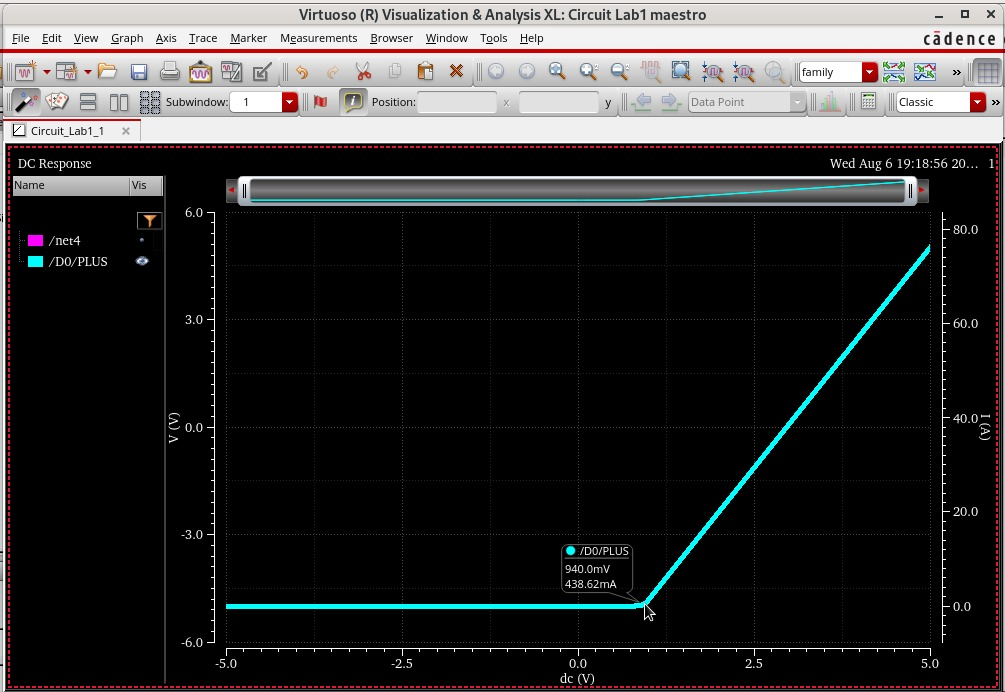
\includegraphics[width=0.7\textwidth]{figs/Diode/Plot.jpg} % Add your image file
    \caption{Plot for Diode I-V Characterization}
\end{figure}

\subsection*{2. BJT I-V Plot}
\begin{figure}[H]
    \centering
    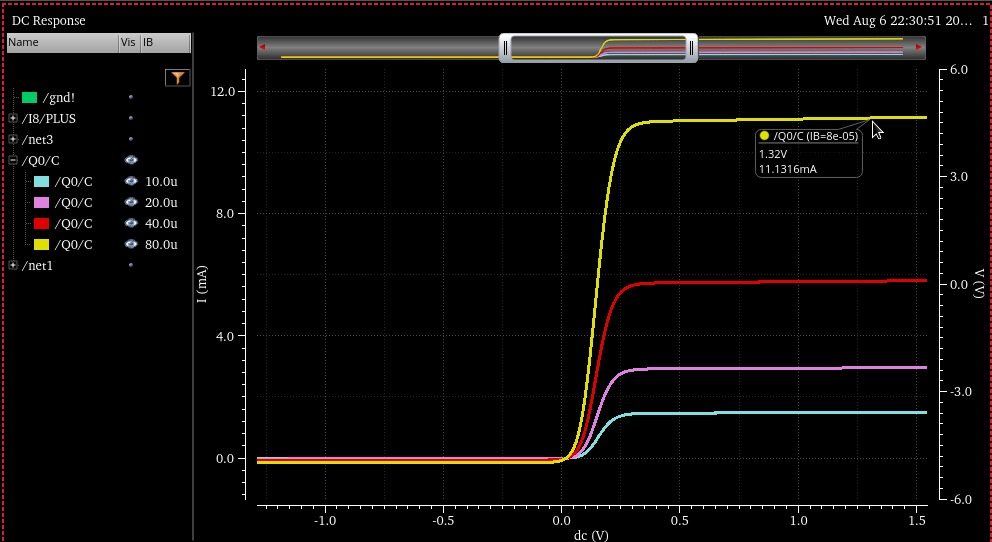
\includegraphics[width=0.7\textwidth]{figs/BJT/NPN/Plot.jpg} % Add your image file
    \caption{Plot for NPN BJT I-V Characterization}
\end{figure}

\begin{figure}[H]
    \centering
    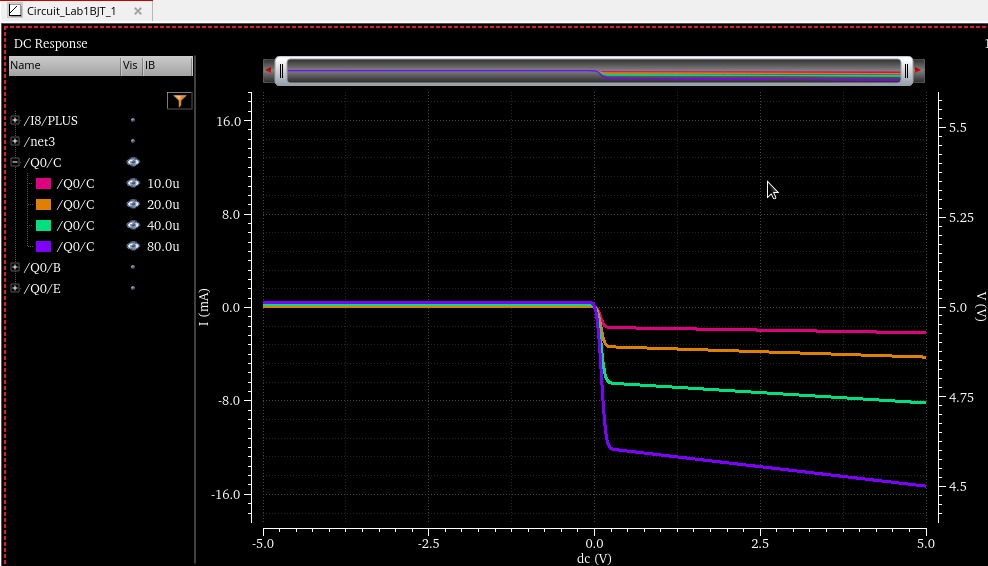
\includegraphics[width=0.7\textwidth]{figs/BJT/PNP/Plot.jpg} % Add your image file
    \caption{Plot for PNP BJT I-V Characterization}
\end{figure}

\subsection*{3. MOSFET I-V Plot}
\begin{figure}[H]
    \centering
    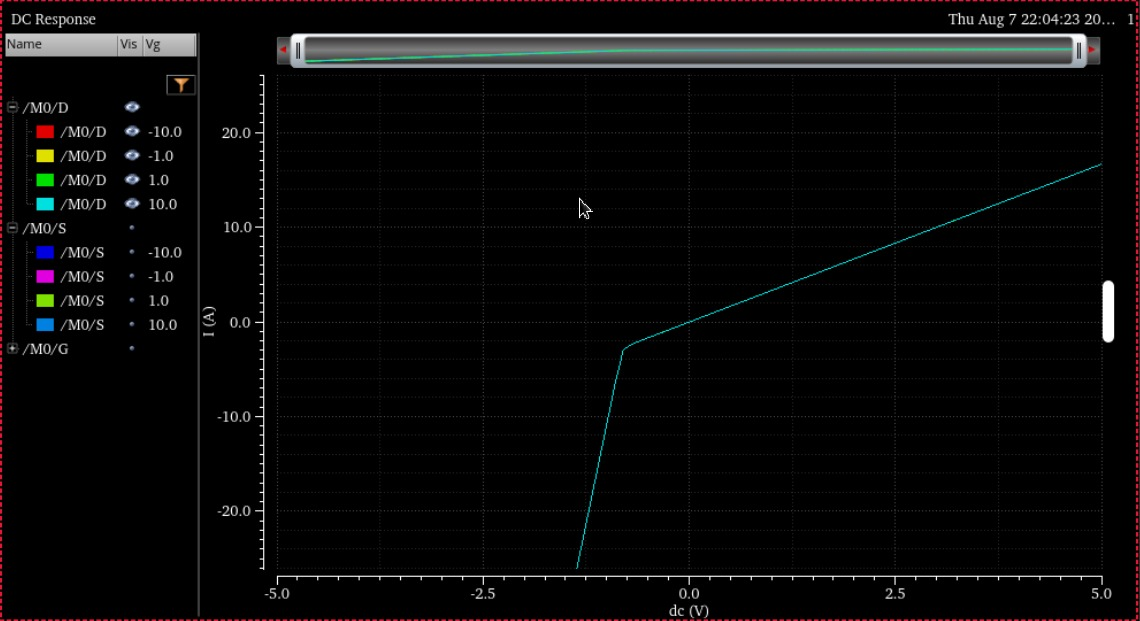
\includegraphics[width=0.7\textwidth]{figs/Mosfet/Plot.jpg} % Add your image file
    \caption{Plot for Mosfet I-V Characterization}
\end{figure}

\section*{Conclusion}
The I-V characteristics of diode, BJT, and MOSFET were successfully simulated using Cadence Virtuoso. The plots align with theoretical expectations:

\begin{itemize}
    \item The diode shows exponential rise in forward bias and negligible reverse current.
    \item The BJT exhibits clear cutoff, active, and saturation regions depending on base current.
    \item The MOSFET demonstrates linear and saturation behavior across various gate voltages.
\end{itemize}

This confirms the accurate modeling and simulation of semiconductor devices using SPICE models and the Cadence Virtuoso platform.
For figs and SpiceModels refer to
\url{}


\centering Thank you!
\end{document}
